
\chapter{Case study}

	\begin{onehalfspace}
	
		This chapter will describe how the application works in a practical approach. To do so, an example showing how to create a fully processed (final) dataset starting from the raw data will be performed. The objective of this final dataset is to be used in ML algorithms to classify waves in the Gulf of Alaska depending on their height.
		
		\section{Case study}
		
		The meteorological data that will be used to perform this case study is described bellow:
		
			\begin{enumerate}
			\item The measurements obtained from 2013 to 2017 by the buoy (46001) placed in the Gulf of Alaska, which are provided by NDBC as annual text files. This data is publicly available at the NDBC website. 
			\item Complementary information collected from reanalysis data containing air temperature, pressure and two components of wind speed (South-North and West-East) measurements. This information will be collected from the four closest reanalysis nodes surrounding the geographical location of the buoy. This data is publicly available at the NNRP website and can be downloaded in NetCDF format.
			\end{enumerate}

			After gathering the information described above \footnote{Further instructions for downloading this data can be found in Appendix \ref{app:GettingMetData}.}, the researcher can open SPAMDA.
			
			In Figure \ref{fig:main_view} the main view can be found, in order to input the reanalysis data which will be used in further steps for creating the final dataset, the researcher will select the option \textcolor{blue}{\textit{Manage reanalysis data}} from the view.
			
			\begin{figure}[ht]
				\centering
				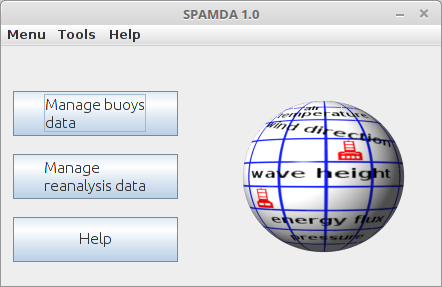
\includegraphics[scale=0.48]{figures/mainView.png}
				\caption{SPAMDA main view.}\label{fig:main_view}
			\end{figure}

			Then, the view represented in Figure \ref{fig:reanalysis} will appear. To enter the four reanalysis files (one per reanalysis variable) the researcher must click on the \textcolor{blue}{\textit{Add reanalysis file}} and a dialog box will appear for selecting them.
			
			\begin{figure}[ht!]
				\centering
				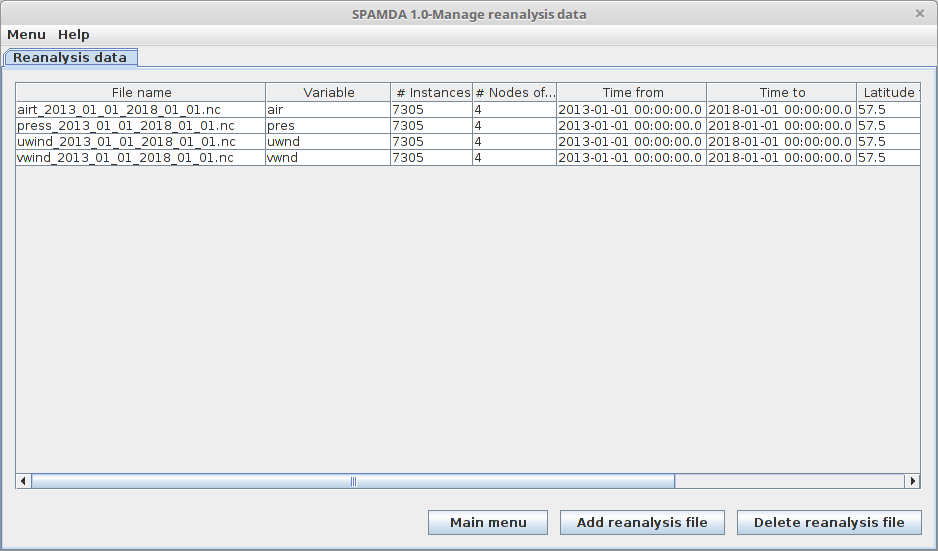
\includegraphics[scale=0.40]{figures/manageReanalysisData_CS.png}
				\caption{Module Manage reanalysis data.}\label{fig:reanalysis}
			\end{figure}
			
			After the reanalysis files has been introduced in SPAMDA, this window can be closed and go back to the main view to continue entering the information related to the buoy under study. The researcher will now select \textcolor{blue}{\textit{Manage buoys data}} to open the view shown in Figure \ref{fig:manage_buoys}. In order to enter such data, click on the \textcolor{blue}{\textit{New}} button, then the window shown in Figure \ref{fig:entering_buoy} will pop-up.
			
			\begin{figure}[ht!]
				\centering
				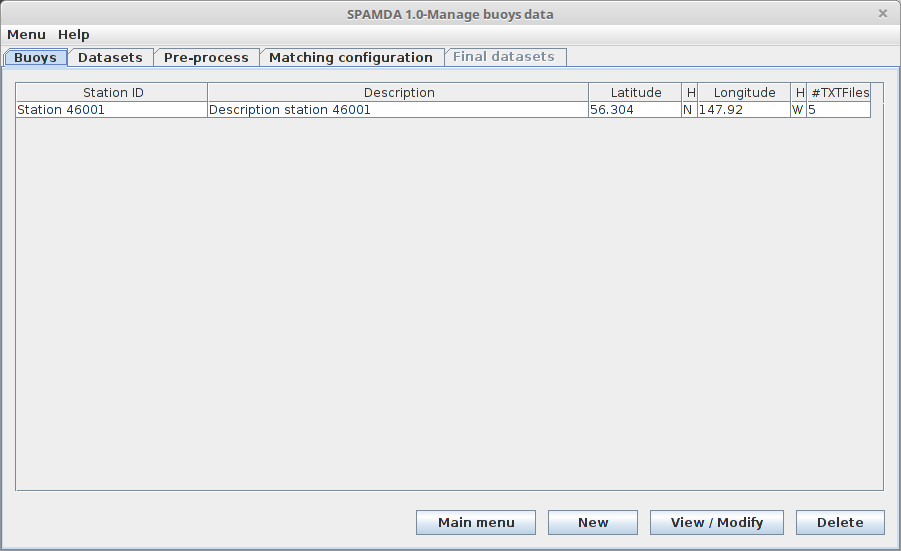
\includegraphics[scale=0.40]{figures/tabBuoys_CS.png}
				\caption{Tab \textit{Buoys}.}\label{fig:manage_buoys}
			\end{figure}

			\begin{figure}[ht!]
				\centering
				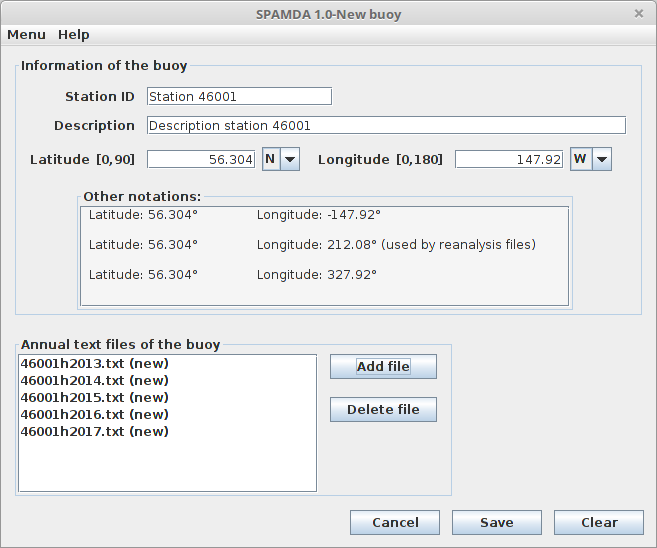
\includegraphics[scale=0.40]{figures/enteringBuoy_CS.png}
				\caption{Entering a new buoy.}\label{fig:entering_buoy}
			\end{figure}

			%Here the information about the buoy will be entered: the \textit{Station ID}, its description, geographical localisation and the corresponding annual text files. In this case, the files containing the data from year $2013$ to $2017$ are inserted. To do so, click on \textcolor{blue}{\textit{Add file}} button and a dialog box will appear for selecting them. Once the data has been introduced, it is necessary to click on \textcolor{blue}{\textit{Save}} button to insert the buoy in SPAMDA database, after that, the window can be closed. To proceed with the creation of the intermediate dataset, double-click on the buoy under study or click on the \textcolor{blue}{\textit{Datasets}} tab to switch to the next view (see Figure \ref{fig:show_datasets}).
			
			Here the information about the buoy will be entered: the \textit{Station ID}, its description, geographical localisation and the corresponding annual text files. In this case, the files containing the data from year $2013$ to $2017$ are inserted. To do so, click on the \textcolor{blue}{\textit{Add file}} button and a dialog box will appear for selecting them. Once the data has been introduced, it is necessary to click on the \textcolor{blue}{\textit{Save}} button to insert the buoy in SPAMDA database, after that, the window can be closed.

			\begin{figure}[ht!]
				\centering
				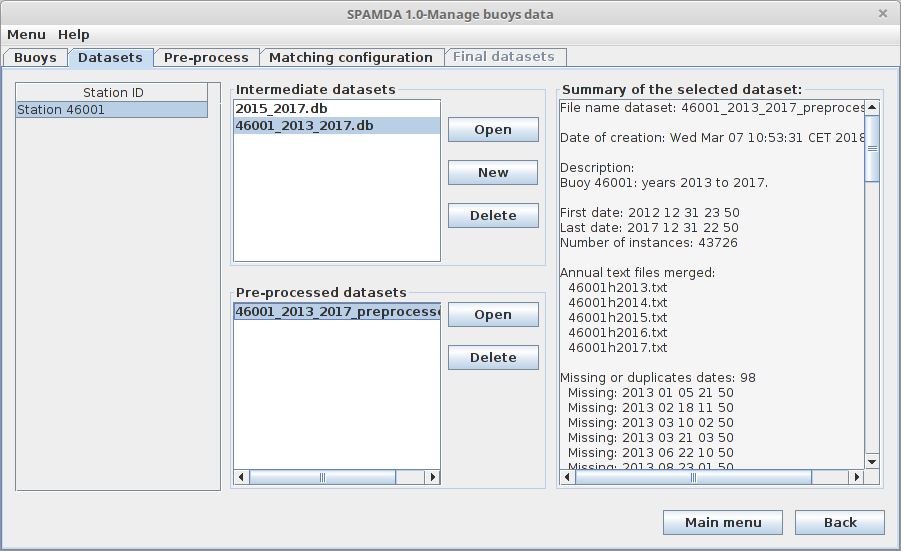
\includegraphics[scale=0.47]{figures/tabDatasets_CS.png}
				\caption{Tab \textit{Datasets}.}\label{fig:show_datasets}
			\end{figure}
			
			%The next step would be to create an intermediate dataset, the researcher will double-click on the buoy under study or click on the \textcolor{blue}{\textit{Datasets}} tab to switch to the next view (see Figure \ref{fig:show_datasets}). In this view, the researcher can delete or consult a brief of each intermediate or pre-processed dataset by selecting it from the corresponding list and also create new ones. To proceed with the creation of the intermediate dataset, click on the \textcolor{blue}{\textit{New}} button and the view shown in Figure \ref{fig:intermediate} will appear.
			
			The next step would be to create an intermediate dataset, the researcher will double-click on the buoy under study or click on the \textcolor{blue}{\textit{Datasets}} tab to switch to the next view (see Figure \ref{fig:show_datasets}).
			
			To proceed with the creation of the intermediate dataset, click on the \textcolor{blue}{\textit{New}} button and the view shown in Figure \ref{fig:intermediate} will appear. 
			
			%The next step would be to create an intermediate dataset including the desired annual text files of the buy. To do so, the researcher can click on \textcolor{blue}{\textit{New}} button and the view shown in Figure \ref{fig:intermediate} will appear.
			
			\begin{figure}[ht!]
				\centering
				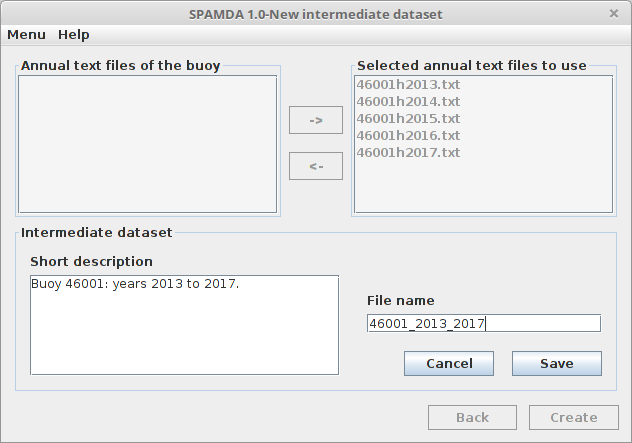
\includegraphics[scale=0.43]{figures/creatingIntermediateDataset_CS.png}
				\caption{New intermediate dataset view.}\label{fig:intermediate}
			\end{figure}
			
			Here the researcher can select the annual text files that he wants to include in the intermediate dataset by clicking on the \textcolor{blue}{\textit{$-$$>$}} button (click on the \textcolor{blue}{\textit{$<$$-$}} button to deselect a previously selected one). In this case, all the files introduced before which correspond to the buoy under study were selected. When the files selection is finished, \textcolor{blue}{\textit{Create}} button will be clicked in order to be able to introduce the description and the file name of the current intermediate dataset, and then clicking on the \textcolor{blue}{\textit{Save}} button, the creation process will start, and the application will show the status of such process.
			
			\begin{figure}[ht!]
				\centering
				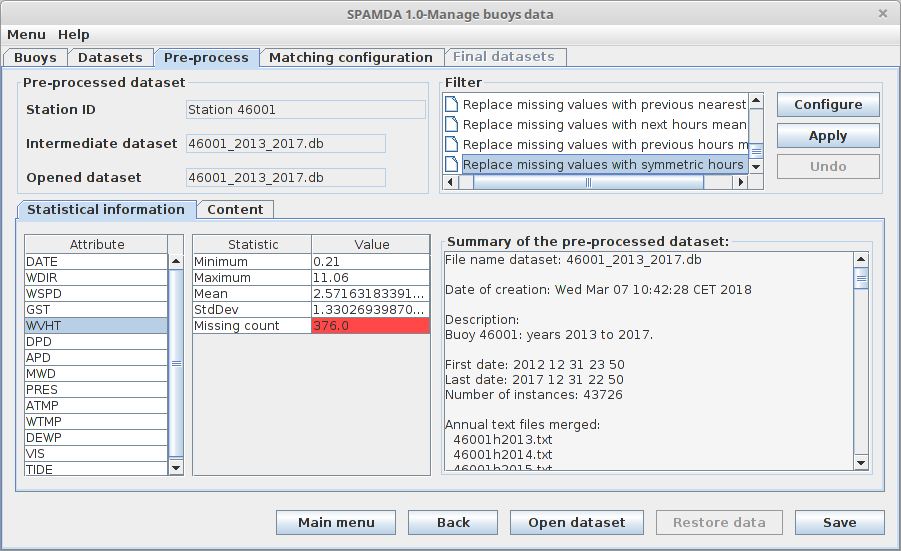
\includegraphics[scale=0.40]{figures/tabPreprocess_CS.png}
				\caption{Tab \textit{Pre-process}.}\label{fig:preprocess_data}
			\end{figure}
			
			%After that, in order to prepare the intermediate dataset to be able to be used by ML algorithms correctly, the dataset to be prepared is selected, and then the button \textcolor{blue}{\textit{Open}} is clicked to jump to the tab \textcolor{blue}{\textit{Pre-process}} (represented in Figure \ref{fig:preprocess_data}). In this tab, relevant statistical information about the selected dataset is shown, and also the content of the dataset can be consulted, providing the researcher the capacity to evaluate the pre-processing being performed.
			
			After that, in order to prepare the intermediate dataset to be able to be used by ML algorithms correctly, the dataset to be prepared is selected, and then the button \textcolor{blue}{\textit{Open}} is clicked to jump to the tab \textcolor{blue}{\textit{Pre-process}} (represented in Figure \ref{fig:preprocess_data}).

			%As mentioned at the beginning of this chapter, this case study will process the data to be ready to classify waves considering their height, so any missing data from wave height ($376$ values) was recovered and some filters were applied to the remaining variables. After finishing the pre-processing of the dataset, the researcher can click on the \textcolor{blue}{\textit{Save}} button, to introduce the description and file name for the current pre-processed dataset.
			
			As mentioned at the beginning of this chapter, this case study will process the data to be ready to classify waves considering their height, so any missing data from wave height ($376$ values) and the remaining attributes are recovered, using the filter \textit{Replace missing values with symmetric $3$ hours mean}. Furthermore, the attributes MWD, DEWP, VIS and TIDE are removed from the dataset by applying the filter \textit{RemoveByName}, since the first two had more than $92$\% of missing data and the last two $100$\%. After finishing the pre-processing of the dataset, the researcher can click on the \textcolor{blue}{\textit{Save}} button, to introduce the description and file name for the current pre-processed dataset.
			
			At this point, the researcher has registered the buoy in SPAMDA, then entered its raw data and selected the required data for the problem (intermediate dataset), finally, the data was pre-processed in order to be ready for its future use in ML algorithms. In order to achieve a more accurate description of the problem under study, a matching process can be carried out to merge the processed data from NDBC with the reanalysis data (also entered previously) from NNRP. The next step is to click on the \textcolor{blue}{\textit{Matching configuration}} tab, to open the view shown in  Figure \ref{fig:matching_conf}. 
			
			\begin{figure}[ht!]
				\centering
				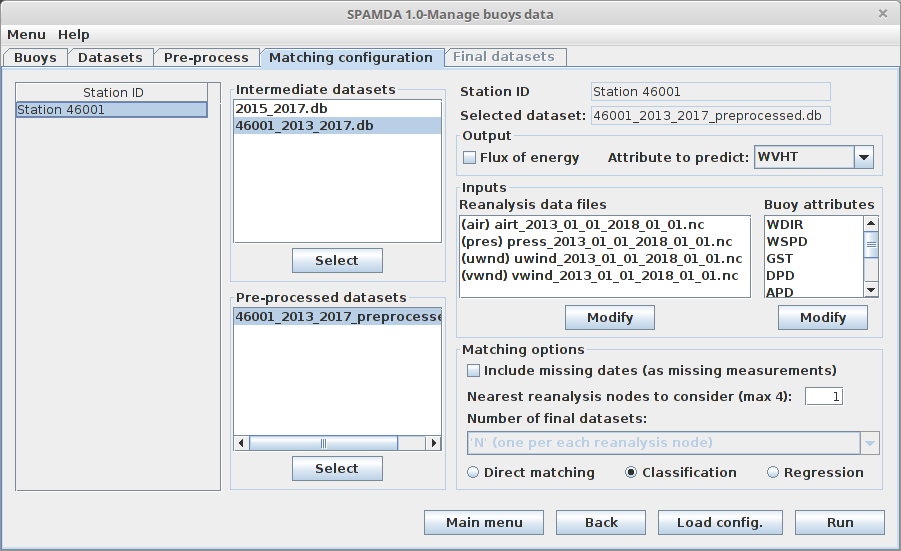
\includegraphics[scale=0.40]{figures/tabMatchingConfiguration_CS.png}
				\caption{Tab \textit{Matching configuration}.}\label{fig:matching_conf}
			\end{figure}
			
			In this view, the researcher can customise (or load) the parameters of the matching process according to his needs, and select the prediction task (described in Section \ref{sec:MatchingConf}) that the final dataset will be used in. For this example the pre-processed dataset created and the following parameters were selected:
			\begin{itemize}
				\setlength\itemsep{0.01cm}
				\item \textit{\textbf{Attribute to predict}}: WVHT.
				\item \textit{\textbf{Reanalysis data}}: Air, pressure, u-wind and v-wind.
				\item \textit{\textbf{Buoy attributes to be used as inputs}}: WDIR, WSPD, GST, DPD, APD, PRES, ATMP and WTMP.
				\item \textit{\textbf{Reanalysis nodes to consider}}: $1$.
				\item \textit{\textbf{Number of final datasets}}: In this example that option is disabled because only 1 reanalysis node is considered.
				\item \textit{\textbf{Prediction task}}: Classification.
			\end{itemize} 

			After configuring the matching process, the researcher can click on the \textcolor{blue}{\textit{Run}} button to jump to the view shown in Figure \ref{fig:final_dataset} and proceed to define the final dataset structure according to the selected prediction task.
			
			\begin{figure}[ht!]
				\centering
				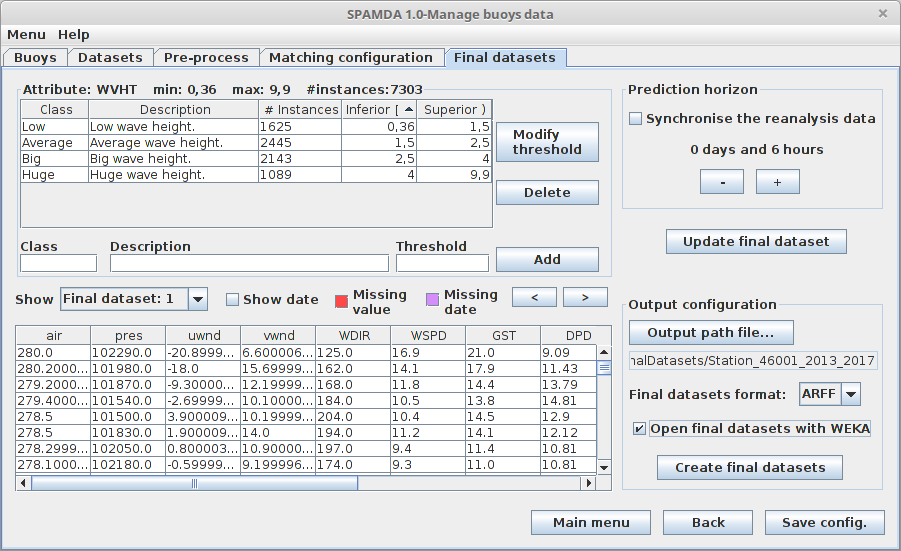
\includegraphics[scale=0.40]{figures/tabFinalDatasets_CS.png}
				\caption{Tab \textit{Final datasets}.}\label{fig:final_dataset}
			\end{figure}
			
			As in the previous window \textit{Classification} was selected, now the researcher is able to add, modify or delete the thresholds (usually defined by an expert) used to discretise the output variable. After adding the necessary thresholds, the next step is to set the time horizon desired and also to activate (if desired) the synchronisation (in time) of reanalysis variables with the output one as explained in Section {\ref{sec:FinalDatasets}}. Then the researcher would click on the \textcolor{blue}{\textit{Update final dataset}} button to see the content of the final dataset which is shown in the bottom left corner and finally, after checking that everything is correct, the last step would be to select the name (and path) of the dataset file, its output format and click on the \textcolor{blue}{\textit{Create final datasets}} button. For this case study the following configuration was applied:
			\vspace{-0.25cm}
			\begin{table}[ht!]
			
				\caption{Defined thresholds.}
				\label{tab:thresholds}
				\footnotesize
				\centering

				\begin{tabular}{cm{3.20cm}cc@{\setlength{\tabcolsep}{0pt}}m{0.0cm}}
				
					\cline{1-5}
					
					\textbf{Class}&\textbf{Description}&\textbf{Inferior [}&\textbf{Superior )}&\\[0.20cm]

					\cline{1-5}
					
					Low & Low wave height & $0.36$ & $1.5$&\\[0.15cm]
					
					\cellcolor{gray090}Average & \cellcolor{gray090}Average wave height & \cellcolor{gray090}$1.5$ & \cellcolor{gray090}$2.5$&\\[0.15cm]
					
					Big & Big wave height & $2.5$ & $4.0$&\\[0.15cm]
					
					\cellcolor{gray090}Huge & \cellcolor{gray090}Huge wave height & \cellcolor{gray090}$4.0$ & \cellcolor{gray090}$9.9$&\\[0.02cm]

					\cline{1-5}
						
				\end{tabular}
			
			\end{table}

			\begin{itemize}
				\item Thresholds: see in Table \ref{tab:thresholds}.
				\item Prediction horizon: 6 hours
				\item Synchronisation: Disabled
			\end{itemize}
			
			At this point the final dataset would be created and stored in the computer of the researcher. Also there is an option to open the dataset with WEKA (after creating it) in order to perform a first classification approach or a preliminary study of the data structure, as shown in Fig. \ref{fig:openigFinalDatasetWekaCE}.

			\begin{figure}[ht!]
				\centering
				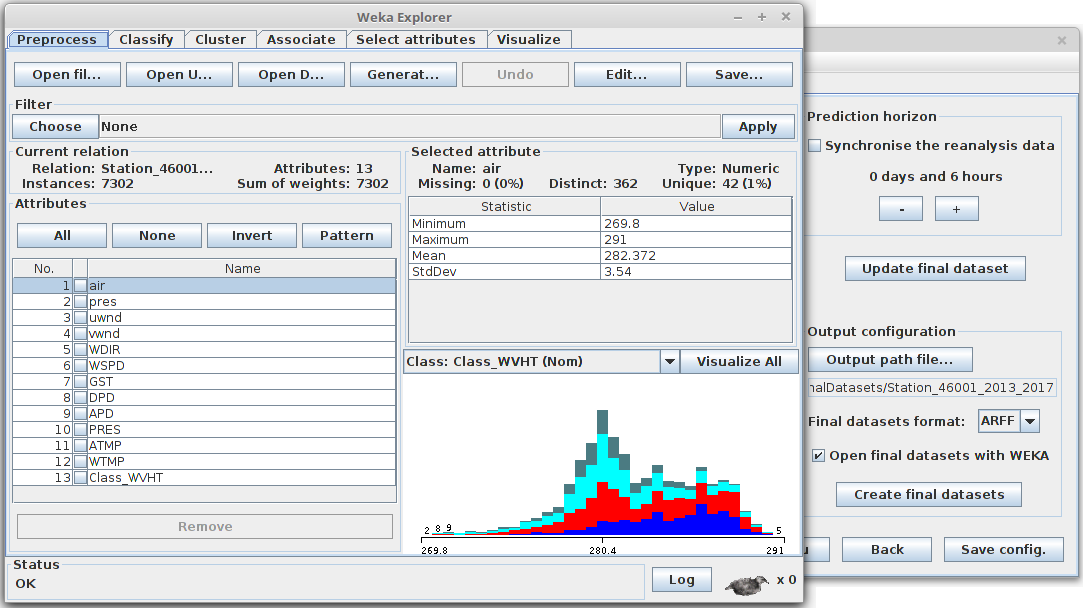
\includegraphics[scale=0.39]{figures/openigFinalDatasetWekaCE.png}
				\caption{The final dataset opened with the environment Explorer of WEKA.}
				\label{fig:openigFinalDatasetWekaCE}
			\end{figure}

	\end{onehalfspace}
	